\documentclass{beamer}
\ifxetex
 \usepackage{fontspec}
\else
 \usepackage[T1]{fontenc}
 \usepackage[utf8]{inputenc}
 \usepackage{lmodern}
\fi
\usepackage{amsmath, pdfpages, pdflscape, lscape, color, listings, hyperref, amssymb,graphicx,textcomp,varioref,afterpage,subcaption, float,color} 


% \makeatletter
% \def\input@path{{/home/simen/Dropbox/phd/presentations/presentations/neuronify}}
% %or: \def\input@path{{/path/to/folder}{/path/to/other/folder}}
% \makeatother

\title{Neuronify: a new tool for creating simple neural networks}
\author{Simen Tennøe,\newline Svenn-Arne Dragly,\newline Andreas V. Solbr\aa,\newline Milad H. Mobarhan}

\usetheme{cinpla3}


\begin{document}
\maketitle

\begin{frame}
  \frametitle{In this lecture we will introduce Neuronify, a new tool for creating neural networks}

  \begin{tikzpicture}[remember picture,overlay]  
    \node [xshift=-3.5cm,yshift=1.5cm] at (current page.center)
          {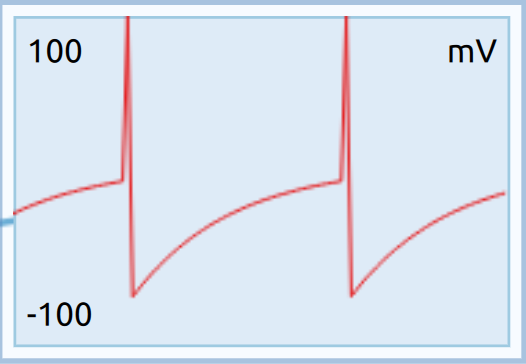
\includegraphics[width = 0.14\paperwidth ]{integrate.png}};
    \node [xshift=-2.cm,yshift=1.5cm, right] at (current page.center)
          { Integrate and fire neurons};
  \end{tikzpicture}

  \begin{tikzpicture}[remember picture,overlay]  
    \node [xshift=-2cm,yshift=-.5cm] at (current page.center)
          {
\includegraphics[width = 0.12\paperwidth ]{logo.png}};
    \node [xshift=1cm,yshift=-.5cm, left] at (current page.center)
          { Neuronify };
  \end{tikzpicture}

  \begin{tikzpicture}[remember picture,overlay]  
    \node [xshift=-.5cm,yshift=-2.5cm] at (current page.center)
          {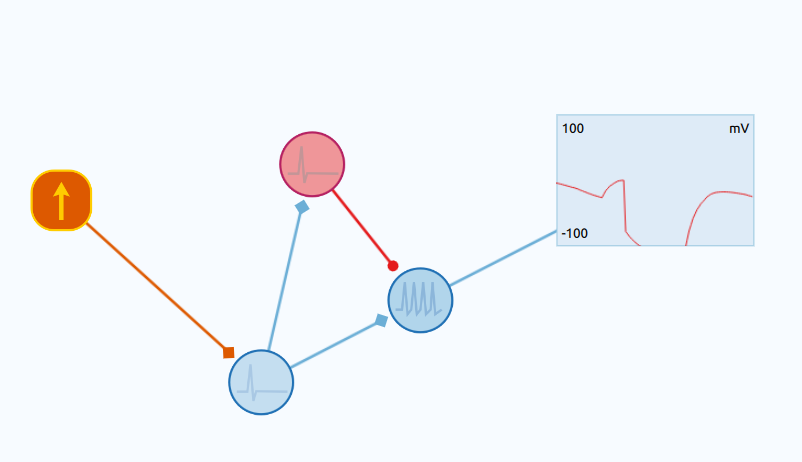
\includegraphics[width = 0.2\paperwidth ]{exercises.png}};
    \node [xshift=2.8cm,yshift=-2.5cm, left] at (current page.center)
          { Exercises};
  \end{tikzpicture}

\end{frame}

\begin{frame}
\frametitle{We do not need all information in the action potential for a neuron in a network and create an approximation of the action potential}
\begin{figure}
\includegraphics<1>[width = \textwidth]{hh.png}
\includegraphics<2>[width = \textwidth]{fi.png}
\end{figure}
\end{frame}


\begin{frame}
\frametitle{The integrate and fire neuron is much faster to evaluate than the Hodgkin-Huxley neuron}

\begin{block}{Hodgkin-Huxley}
\begin{align*}
\onslide<2->  {C\frac{dV}{dt} &= I_{inj} - \bar{g}_{Na}m^3h(V-V_{Na}) -\bar{g}_Kn^4(V-V_K) - g_L (V-V_L)}\\
 \onslide<3->  {\frac{dn}{dt} &= \alpha_n(V) (1-n) - \beta_n(V)n \quad}
 \onslide<4-> {\frac{dm}{dt} = \alpha_m(V) (1-m) - \beta_m(V)m}\\
\onslide<5->  {\frac{dh}{dt} &= \alpha_h(V) (1-h) - \beta_h(V)h \quad}
\onslide<6->  {\alpha_n(V) = \frac{0.01(V+55)}{1-\exp[-(V+55)/10]}} \\
\onslide<7->  {\beta_n(V) &= 1.125\exp[-(V+65)/80] \quad}
\onslide<8->  {\alpha_m(V)  = \frac{0.1(V+40)}{1-\exp[-(V+40)/10]}} \\
\onslide<9->  {\beta_m(V) &= 4\exp[-(V+65)/18] \quad}
\onslide<10->  {\alpha_h(V) = 0.07\exp[-(V+65)/20]} \\
\onslide<11->  {\beta_n(V) &= \frac{1}{1+\exp[-(V+35)/10]}}
\end{align*}
\end{block}

\end{frame}


\begin{frame}
\frametitle{The integrate and fire neuron is much faster to evaluate than the Hodgkin-Huxley neuron}
\begin{block}{Integrate and fire}
\pause
\begin{equation*}
C_m \frac{dV(t)}{dt} = - \frac{V(t) - E_m}{R_m} + I
\end{equation*}
\end{block}

\end{frame}


% \begin{frame}
% \frametitle{The integrate and fire model is modeled as a simple RC circuit that is shortcircuted once a threshold is reached}

% \begin{figure}
% \includegraphics<1>[width = 0.5\textwidth]{rcA.png}
% \includegraphics<2>[width = 0.5\textwidth]{rcAI.png}
% \includegraphics<3>[width = 0.5\textwidth]{rcARm.png}
% \includegraphics<4>[width = 0.5\textwidth]{rcAEm.png}
% \includegraphics<5>[width = 0.5\textwidth]{rcACm.png}
% \includegraphics<6>[width = 0.5\textwidth]{rcAs.png}
% % \includegraphics<7>[width = 0.5\textwidth]{rcB.png}
% % \includegraphics<8>[width = 0.5\textwidth]{rcBs.png}
% \end{figure}
% \end{frame}


\begin{frame}
\frametitle{Neuronify is a new tool for creating neural networks}
\begin{figure}

\includegraphics[height = 0.8\textheight]{logo.png}
\end{figure}
\end{frame}


\begin{frame}
\frametitle{Exercises}
\begin{figure}
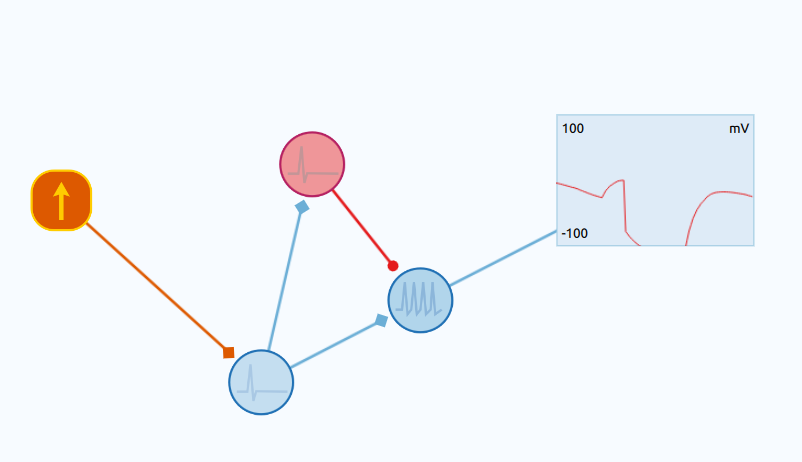
\includegraphics[width = \textwidth]{exercises.png}
\end{figure}
\end{frame}

\end{document}
